\begin{figure}
    \centering
    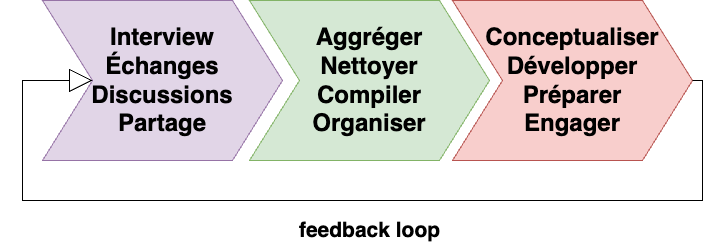
\includegraphics[width=0.75\linewidth]{images/Diagrams-Simplified framework chain Our approach.png}
    \caption{Notre approche simplifiée}
    \label{fig:simplified-approach}
\end{figure}

Notre travail s’inscrit dans l’alliance universitaire européenne UNITA - Universitas Montium, composée de 12 institutions collaborant autour d’objectifs communs. Cette alliance constitue une base d’expérimentation, illustrant les défis auxquels les universités européennes et, plus largement, les méta-organisations font face en matière d’évaluation d’impact sociétal.

Notre approche repose sur un cadre multi-axes aidant les méta-organisations, telles qu’UNITA, à évaluer leur impact via des méthodologies et outils orientés données (Figure~\ref{fig:simplified-approach}). Nous proposons une solution de stockage orientée impact, intégrant la collecte de preuves, l’analyse d’indicateurs et des entretiens collaboratifs.

Les indicateurs d’outputs (résultats immédiats, comme le nombre de projets terminés) et d’outcomes (effets à moyen terme, comme l’accroissement des collaborations) sont au cœur de cette démarche pour suivre les progrès et soutenir la prise de décisions stratégiques.

Notre méthode s’articule en trois étapes : 
\begin{itemize} 
\item \textbf{Discussion} : Identifier les besoins de chaque institution membre. \item \textbf{Évaluation} : Valider des indicateurs fiables et adaptés. 
\item \textbf{Construction} : Intégrer les données validées dans un entrepôt structuré (DWH). 
\end{itemize}

Les données intégrées dans le DWH permettent de générer des rapports d’évaluation, d’identifier les tendances collaboratives et de suivre les progrès. Le nettoyage des données garantit la suppression des doublons et incohérences, assurant ainsi une intégration cohérente et des analyses fiables.

Ce cadre ne se limite pas à mesurer les résultats actuels, mais vise aussi à prédire l’impact futur des actions menées par l’alliance sur son environnement sociétal. Une précision accrue des données améliore directement la performance des modèles de prédiction.